% !TEX TS-program = xelatex

%%%%%%%%%%%%%%%%%%%%%%% 
% 文档类型,页面布局
\documentclass[UTF8,a4paper,10pt]{ctexart}
\usepackage[left=2.50cm, right=2.50cm, top=2.50cm, bottom=2.50cm]{geometry} %页边距
\CTEXsetup[format={\Large\bfseries}]{section} %设置章标题居左

%%%%%%%%%%%%%%%%%%%%%%% 
% 设置中文字体,用 xelatex 编译
% \setmainfont{Microsoft YaHei}  % 微软雅黑
% \setmainfont{YouYuan}  % 幼圆
% \setmainfont{NSimSun}  % 新宋体
% \setmainfont{KaiTi}    % 楷体
% \setmainfont{SimSun}   % 宋体
% \setmainfont{SimHei}   % 黑体

%%%%%%%%%%%%%%%%%%%%%%% 
% 设置英文字体
% \usepackage{times}
% \usepackage{mathpazo}
% \usepackage{fourier}
% \usepackage{charter}
% \usepackage{helvet}

%%%%%%%%%%%%%%%%%%%%%%% 
% 各种包
\usepackage{amsmath, amsfonts, amssymb} % math equations, symbols
\usepackage[english]{babel}
\usepackage{color}      % color content
\usepackage{graphicx}   % import figures
\graphicspath{{figures/}}
\usepackage{url}        % hyperlinks
\usepackage{bm}         % bold type for equations
\usepackage{multirow} 	% multirow
\usepackage{booktabs}	% toprule,midrule,cmidrule,bootomrule
\usepackage{epstopdf}
\usepackage{epsfig}
\usepackage{algorithm}
\usepackage{algorithmic}
\renewcommand{\algorithmicrequire}{ \textbf{Input:}}     % use Input in the format of Algorithm
\renewcommand{\algorithmicensure}{ \textbf{Initialize:}} % use Initialize in the format of Algorithm
\renewcommand{\algorithmicreturn}{ \textbf{Output:}}     % use Output in the format of Algorithm

%%%%%%%%%%%%%%%%%%%%%%% 
%% lstings for Source code
\input{listings.setting}

%%%%%%%%%%%%%%%%%%%%%%% 
% 设置超链接,书签
\usepackage[
bookmarksnumbered=true,
bookmarksopen=false,
bookmarksopenlevel=1,
colorlinks=true,  % it must be enabled to enable other color option
citecolor=blue,
filecolor=green,
linkcolor=blue,
urlcolor=red,
pdfstartview=Fit
]{hyperref}


%%%%%%%%%%%%%%%%%%%%%%% 
% 设置页眉、页脚
\usepackage{fancyhdr}
% \pagestyle{fancy}
\lhead{}
\chead{}
% \rhead{\includegraphics[width=1.2cm]{fig/ZJU_BLUE.eps}}
\lfoot{}
\cfoot{}
\rfoot{}

%%%%%%%%%%%%%%%%%%%%%%% 
% 设置水印
% \usepackage{draftwatermark}         % 所有页加水印
% \usepackage[firstpage]{draftwatermark} % 只有第一页加水印
% \SetWatermarkText{Water-Mark}           % 设置水印内容
% \SetWatermarkText{\includegraphics{fig/ZJDX-WaterMark.eps}}         % 设置水印logo
% \SetWatermarkLightness{0.9}             % 设置水印透明度 0-1
% \SetWatermarkScale{1}                   % 设置水印大小 0-1


%%%%%%%%%%%%%%%%%%%%%%%%%%%%%%%%%%%%%%%%%%%%%%%%%%%%%%%%%%%%%%%%%%%%%%%%%%%%%%%% 
% 正文
%%%%%%%%%%%%%%%%%%%%%%%%%%%%%%%%%%%%%%%%%%%%%%%%%%%%%%%%%%%%%%%%%%%%%%%%%%%%%%%% 
\title{
  \textbf{位姿表示}
}
\author{石正璞
  % \thanks{学号:xx2017xxxx} 
}
\date{
  % \today
  2023年11月20日
}

\begin{document}
\maketitle	

\begin{abstract}
  本文以笔记的形式对位姿的相关概念和算法进行了梳理,以定理证明的形式进行了描述,为进一步的算法设计和软件实现提供了基础。
\end{abstract}

\paragraph{Keyword:}位姿,Pose, Position, Orientation


% ##################################################################################################
% \section{引言}

% ##################################################################################################
\section{基本概念}\label{sec:concepts}
我们需要6个维度来完整描述三维世界中一个刚性物体(rigid body)的位姿:位置3个,朝向3个。
这些维度的行为不同:若增加一个位置维度的值,该物体会在直线上连续运动;若增加一个朝向维度的值,该物体会将以某种方式旋转并不久后回到原来的朝向——这个维度是弯曲的(curved)。
显然,我们要以不同的方式来处理位置和朝向的维度。
以下是基本概念。
\begin{itemize}
\item{\textbf{笛卡尔坐标系统}}
  (Cartesian Coordinate System),或称坐标系(Coordinate Frame, Frame),
  是一些正交的(orthogonal)轴的集合,交点称为原点(origin)。
  使用标签来区分不同坐标系,其坐标轴用该标记作为下标。
  例如:物体坐标系(object coordinate frame) 记为{B},其坐标轴记为 $x_B, y_B$。
\item{\textbf{(空间中的)点}}
  是重要的数学概念,可以用一个坐标向量来描述。该向量描述了该点相对于坐标系的位移。
  点与向量是不同类型的数学对象,虽然都能用数字元组来描述。
  可以对向量做加法,但对点做加法没有意义。
  两个点的差是一个向量,对一个点加上一个向量可以得到另一个点。
\item{\textbf{向量}}
  向量可用其分量来描述,它是平行于坐标轴的单位向量的线性组合。
  具有固定起点和终点的向量称为束缚向量(bound vector),或称坐标向量。
  当矢量的大小和方向很重要时,特定的初始点并不重要,并且该矢量称为自由矢量。
\item{\textbf{(空间中的)物体}}
  由无穷多的点构成。物体与点不同,它还有朝向(也称方向)。
  当给物体附加一个坐标系时,该物体内所有点都可描述为关于这个坐标系的常向量。
\item{\textbf{位姿}}
  (pose)是指物体(相对于参考坐标系的)坐标系的位置和朝向。
  相对位姿是一个坐标系相对于另一个参考坐标系的位姿。
  坐标系的位姿用 $\xi$表示,相对位姿${}^A\xi_B$表示坐标系{B}相对于{A}的位姿。
  一个点的坐标向量可以用另一个不同的坐标系来表示,通过使用$\cdot$运算将相对位姿作用到该向量上。
  多个三维坐标系与相对位姿的例子如图\eqref{fig:multiple_frame_pose}。
  \begin{figure}[htbp]
    \centerline{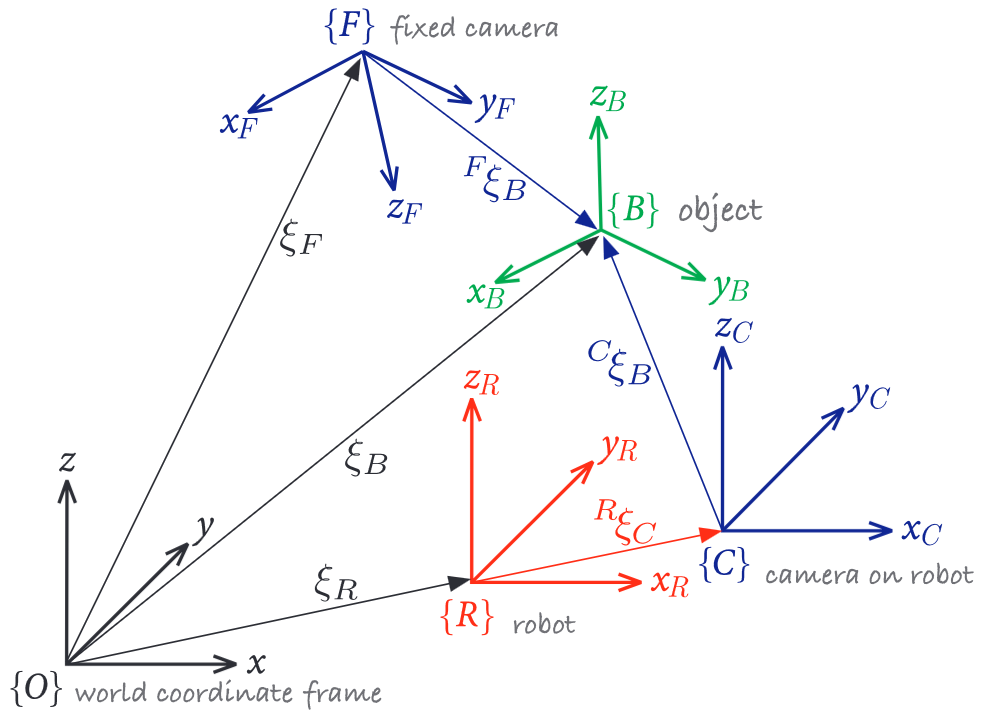
\includegraphics[width=0.9\textwidth]{multiple_frame_pose}}
    \caption{多个三维坐标系与相对位姿的例子}
    \label{fig:multiple_frame_pose}
  \end{figure}
  这些空间关系还可以用有向图来表示,如图\ref{fig:pose_directed_graph}。
  \begin{figure}[htbp]
    \centerline{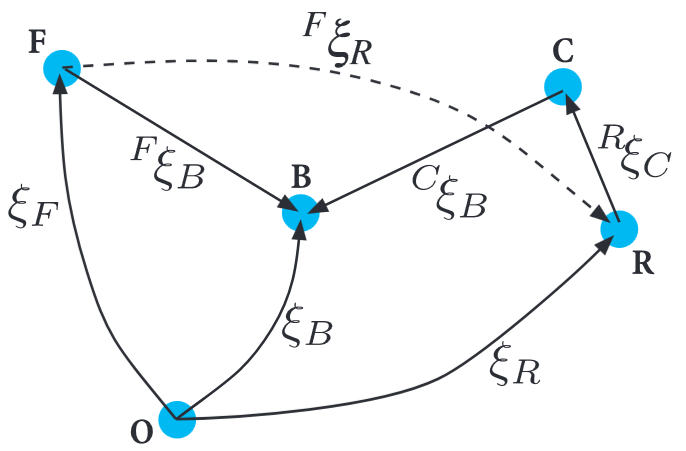
\includegraphics[width=0.9\textwidth]{pose_directed_graph}}
    \caption{有向图表示的空间关系}
    \label{fig:pose_directed_graph}
  \end{figure}
  
\item{\textbf{特殊欧式群}}
  特殊欧式群(special Euclidean group),在二维和三维中分别记为SE(2)和SE(3)。
  群元素是位姿(即满足某种条件的2维或3维矩阵),它满足结合律,有单位元,逆元。
  记该群为 $\langle G,\oplus,0,\ominus\rangle$,其抽象的运算规则如下:
  \begin{itemize}
  \item {相对位姿可以把一个点在某个坐标系下的向量表示转换到另一个坐标系下},${}^Xp={}^X\xi_Y\cdot{}^Yp$。
  \item{位姿可以复合},${}^X\xi_Y\oplus{}^Y\xi_Z={}^X\xi_Z$。
  \item{零相对位姿,$0$}。
  \item{每个元素都有逆元},$\ominus{}^X\xi_Y={}^Y\xi_X$。
  \item{一些代数规则},
    $
    \xi\oplus0=\xi,\quad0\oplus\xi=\xi,\quad\xi\oplus(\ominus\xi)=0,\quad(\ominus\xi)\oplus\xi=0.
    $
  \item {复合运算不交换},$\xi_1\oplus\xi_2\ne\xi_2\oplus\xi_1$。
    一个例外是当$\xi_1\oplus\xi_2=0$时。
  \end{itemize}
  另外,该群具有执行代数的能力。
  一方面,群都满足消去律,所以可以化简等式。
  另一方面,可快速找到任意节点$X$相对于节点$Y$的位姿,步骤为:
  \begin{enumerate}
  \item 找到一条从$Y$到$X$的路径,在边上从左到右的写下相对位姿;
  \item 如果所经过的边与箭头方向相同则在前面冠以$\oplus$,否则冠以$\ominus$。
  \end{enumerate}
  例如,若要计算$R$相对于$F$的位姿${}^F\xi_R$,有多个路径可选。
  当选择$F,O,R$时,获得的相对位姿是$\ominus\xi_F\oplus\xi_R$。
  当选择$F,B,C,R$时,获得的相对位姿是$\oplus{}^F\xi_B\ominus{}^C\xi_B\ominus{}^R\xi_C$。
\item{\textbf{位姿$\xi$到底是什么?}}
  它是一种能够满足上述代数运算的任何数学对象。
  接下来会介绍。
  熟悉的概念包括向量等。
  其他的将是更奇特的数学对象,例如齐次变换、正交旋转矩阵、扭曲和四元数。
\end{itemize}

% ##################################################################################################
\section{二维情形}\label{sec:2D}

对于二维世界(或称平面),我们非常熟悉。
使用笛卡尔坐标系统,或带有两个正交轴(典型的记为$x$和$y$)的坐标系。
平行于坐标轴的单位向量记为$\hat{\mathbf{x}}$和$\hat{\mathbf{y}}$。
一个点用它的$x-$和$y-$坐标$(x,y)$来表示,或者作为一个约束向量
\begin{equation}\label{eq:point2D}
  \mathbf{p}=x\hat{\mathbf{x}}+y\hat{\mathbf{y}}
\end{equation}

如图\ref{fig:two_frame_2D}所示,给定了红色坐标系${B}$,我们要描述它关于蓝色坐标系${A}$的位姿。
其中,${B}$的原点被移动了向量$t=(x,y)$,然后${B}$又逆时针旋转了$\theta$角。
\begin{figure}[htbp]
  \centerline{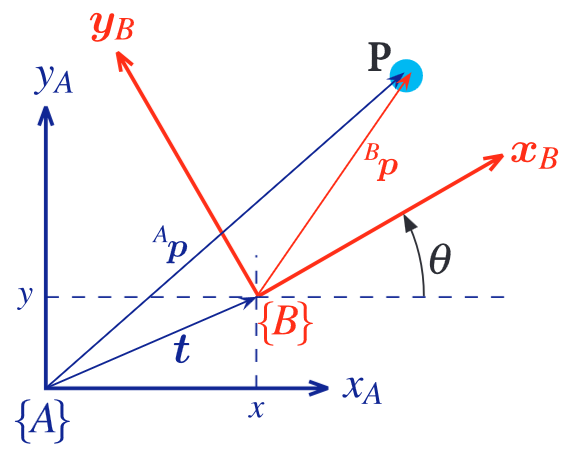
\includegraphics[width=0.6\textwidth]{two_frame_2D}}
  \caption{平面上的任意两个坐标系}
  \label{fig:two_frame_2D}
\end{figure}
一种方法是使用三维向量${}^A\xi_B\sim(x,y,\theta)$,其中符号$\sim$表示这两个表示等价。
但是,这种表示不方便,因为两个位姿的复合$(x_1,y_1,\theta_1)\oplus(x_2,y_2,\theta_2)$是复杂的三角函数。
我们将把问题分为两部分:旋转,然后平移。

\subsection{二维中的朝向}
\subsubsection{标准正交旋转矩阵(Orthonomal Rotation Matrix)}

如图\ref{fig:two_frame_2D}所示,任意点$P$可以相对于每个坐标系而表示。
新建一个坐标系$\{V\}$,其坐标轴与$\{A\}$的平行,原点与$\{B\}$的相同,如图\ref{fig:two_frame_2D_V}所示。
\begin{figure}[htbp]
  \centerline{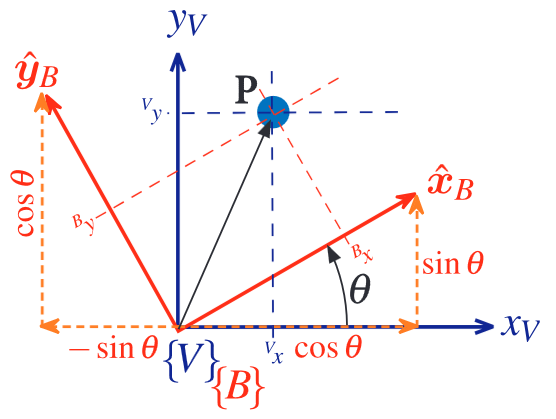
\includegraphics[width=0.6\textwidth]{two_frame_2D_V}}
  \caption{辅助坐标系$\{V\}$}
  \label{fig:two_frame_2D_V}
\end{figure}

点$P$相对于$\{V\}$和$\{B\}$可以用其分别的坐标轴单位向量来表示
\begin{equation}\label{eq:pV}
  {}^V\mathbf{p}={}^Vx\hat{\mathbf{x}}_V + {}^Vy\hat{\mathbf{y}}_V =
  \begin{pmatrix}\hat{\mathbf{x}}_V&\hat{\mathbf{y}}_V\end{pmatrix}
  \begin{pmatrix}{}^Vx\\{}^Vy\end{pmatrix}
\end{equation}
\begin{equation}\label{eq:pB}
  {}^B\mathbf{p}={}^Bx\hat{\mathbf{x}}_B + {}^By\hat{\mathbf{y}}_B =
  \begin{pmatrix}\hat{\mathbf{x}}_B&\hat{\mathbf{y}}_B\end{pmatrix}
  \begin{pmatrix}{}^Bx\\{}^By\end{pmatrix}
\end{equation}

坐标系$\{B\}$可完全由它的两个正交轴所描述,而这两个轴的单位向量与坐标系$\{V\}$的坐标轴单位向量之间有如下关系
\begin{align*}
  \hat{\mathbf{x}}_B&=\cos\theta\hat{\mathbf{x}}_V + \sin\theta\hat{\mathbf{y}}_V\\
  \hat{\mathbf{y}}_B&=-\sin\theta\hat{\mathbf{x}}_V + \cos\theta\hat{\mathbf{y}}_V
\end{align*}
其矩阵形式为
\begin{equation}\label{eq:unitVecV2B_raw}
  \begin{pmatrix}\hat{\mathbf{x}}_B&\hat{\mathbf{y}}_B\end{pmatrix}=
  \begin{pmatrix}\hat{\mathbf{x}}_V&\hat{\mathbf{y}}_V\end{pmatrix}
  \begin{pmatrix}\cos\theta  & -\sin\theta\\\sin\theta & \cos\theta\end{pmatrix}
\end{equation}
将式\eqref{eq:unitVecV2B_raw}带入\eqref{eq:pB},得到如下形式
\begin{equation}\label{eq:pB2}
  {}^B\mathbf{p}={}^Bx\hat{\mathbf{x}}_B + {}^By\hat{\mathbf{y}}_B =
  \begin{pmatrix}\hat{\mathbf{x}}_V&\hat{\mathbf{y}}_V\end{pmatrix}
  \begin{pmatrix}\cos\theta  & -\sin\theta\\\sin\theta & \cos\theta\end{pmatrix}
  \begin{pmatrix}{}^Bx\\{}^By\end{pmatrix}
\end{equation}
由于${}^V\mathbf{p}$和${}^B\mathbf{p}$实际上是同一个向量,所以\eqref{eq:pV}和\eqref{eq:pB2}的右侧是同一个向量。
又因为此时它们用同一个基向量$\begin{pmatrix}\hat{\mathbf{x}}_V&\hat{\mathbf{y}}_V\end{pmatrix}$来表示,所以其对应系数相等。
\begin{equation}\label{eq:xyB2V_raw}
  \begin{pmatrix}{}^Vx\\{}^Vy\end{pmatrix}=
  \begin{pmatrix}\cos\theta  & -\sin\theta\\\sin\theta & \cos\theta\end{pmatrix}
  \begin{pmatrix}{}^Bx\\{}^By\end{pmatrix}
\end{equation}
记
\begin{equation}\label{eq:RBV}
  {}^V\mathbf{R}_B=
  \begin{pmatrix}\cos\theta  & -\sin\theta\\\sin\theta & \cos\theta\end{pmatrix}
\end{equation}
称\eqref{eq:RBV}中的矩阵${}^V\mathbf{R}_B$是一个旋转矩阵,它表示坐标系$\{V\}$是由$\{B\}$绕原点旋转了$\theta$而来。
此时,\eqref{eq:unitVecV2B_raw}和\eqref{eq:xyB2V_raw}得到更紧凑的形式
\begin{equation}\label{eq:unitVecV2B}
  \begin{pmatrix}\hat{\mathbf{x}}_B&\hat{\mathbf{y}}_B\end{pmatrix}=
  \begin{pmatrix}\hat{\mathbf{x}}_V&\hat{\mathbf{y}}_V\end{pmatrix}
  {}^V\mathbf{R}_B
\end{equation}
\begin{equation}\label{eq:xyB2V}
  \begin{pmatrix}{}^Vx\\{}^Vy\end{pmatrix}=
  {}^V\mathbf{R}_B
  \begin{pmatrix}{}^Bx\\{}^By\end{pmatrix}
\end{equation}
式\eqref{eq:unitVecV2B}描述了如何将坐标轴向量从坐标系$\{V\}$转换到$\{B\}$下(即,右乘矩阵${}^V\mathbf{R}_B$)。
式\eqref{eq:xyB2V}描述了如何将点从坐标系$\{B\}$转换到$\{V\}$下(即,左乘矩阵${}^V\mathbf{R}_B$)。

任给二维旋转矩阵${}^Y\mathbf{R}_X$,具有一些特殊性质
\begin{itemize}
\item 它是正规的、标准正交的(orthonormal),简称正交的(orthogonal)。
  因为每一列是单位向量,并且列之间是正交的。
\item 列向量定义了旋转后的坐标系$\{Y\}$在坐标系$\{X\}$下的轴向量。
\item 它属于二维特殊正交群,即$\mathbf{R}\in\mathbf{SO}(2)\subset\mathbb{R}^{2\times2}$。
  这意味着,任意两个该群的矩阵相乘仍在群中,其逆也在群中。
\item 它的行列式是$+1$,这表明向量在变换之后长度不改变。
  即,$\|{}^Y\mathbf{p}\|=\|{}^X\mathbf{p}\|, \forall\theta$
\item 其逆矩阵等于其转置,即,$\mathbf{R}^{-1}=\mathbf{R}^{T}$。
\end{itemize}

对\eqref{eq:xyB2V}变形,得到
\begin{equation*}
  \begin{pmatrix}{}^Bx\\{}^By\end{pmatrix}=
  \left({}^V\mathbf{R}_B\right)^{-1}\begin{pmatrix}{}^Vx\\{}^Vy\end{pmatrix}=
  \left({}^V\mathbf{R}_B\right)^{T}\begin{pmatrix}{}^Vx\\{}^Vy\end{pmatrix}=
  {}^B\mathbf{R}_V\begin{pmatrix}{}^Vx\\{}^Vy\end{pmatrix}
\end{equation*}
可知逆矩阵与交换矩阵上下标是一样的,即
\begin{equation}
  \left({}^V\mathbf{R}_B\right)^{-1}={}^B\mathbf{R}_V
\end{equation}
另外,很容易验证
\begin{equation}
  \mathbf{R}(-\theta)=\mathbf{R}(\theta)^T
\end{equation}

一个有趣的观察是,我们不使用一个标量的角度作为参数,而是使用由4个元素构成的$2\times2$矩阵。
尽管这些元素并不独立。
每列都具有单位大小提供了2个约束,列是正交的提供了另一个约束,于是4个元素在3个约束下必然是一个独立的值。
旋转矩阵是非最小表示(nonminimum representation)的一个例子,其缺点是增加了存储空间,而优点是提供了可组合性(即矩阵乘法)。

在MATLAB中的实验。
\begin{matlab}
  % 创建了一个旋转矩阵
  R = rot2(0.2)
  % 行列式是1
  det(R)
  % 相乘仍然是旋转矩阵
  det (R*R)
  % 还支持符号数学
  syms theta
  R = rot2(theta)
  simplify(R*R)
  simplify(det(R))
\end{matlab}

\subsubsection{矩阵指数}
二维中的斜对称矩阵(skew-symmetric matrix)是指满足$-\mathbf{M}=\mathbf{M}^T$的矩阵,其一般形式为
\begin{equation}
  [\omega]_{\times}=
  \begin{bmatrix}0&-\omega\\\omega&0\end{bmatrix},
\end{equation}
其中,$\omega\in\mathbb{R}$。

在MATLAB中的实验。
\begin{matlab}
  % 数值 -> 斜对称阵
  R=skew(2)
  % 斜对称阵 -> 数值
  x=vex(R)
  % 一个0.3弧度的纯旋转表示为旋转矩阵
  R=rot2(0.3)
  % 使用矩阵对数求得另一个矩阵S
  S=logm(R)    % S是斜对称矩阵,对应于实数0.3,巧合吗?
  % 矩阵指数是矩阵对数的逆
  R1=expm(S)   % 得到的R1等于R
\end{matlab}
上述的这种巧合来源于李群(Lie group)理论。

矩阵指数(exponentiation)的逆是矩阵对数(logarithm of the matrix)。
在MATLAB中,使用\verb|expm(x)|和\verb|logm(x)|函数来计算矩阵指数和矩阵对数。
事实上,在RVC中\verb|rot2|被定义为\verb|rot2(x)=expm(skew(x))|。

矩阵指数的计算公式为:
$$
\mathtt{expm}(\mathbf{A})
=\sum_{n=0}^{\infty}\frac{\mathbf{A}^n}{n!}
=\mathbf{I}+\mathbf{A}+\frac{\mathbf{A}^2}{2!}+\frac{\mathbf{A}^3}{3!}+\ldots
$$
形式上,写作
$$
\mathbf{R}(\theta)=e^{[\theta]_{\times}}\in\mathbf{SO}(2)
$$
因为指数函数的幂级数是
$$
e^{x}=\sum_{n=0}^{\infty}\frac{x^n}{n!}=1+x+\frac{x^2}{2!}+\frac{x^3}{3!}+\ldots
$$

提示,MATLAB默认实数显示4位小数,在预设/命令行窗口/文本显式/数值格式,可把short修改为long来显示15位小数。

\subsection{二维中的位姿}

\subsubsection{齐次变换矩阵}

一个向量$\mathbf{p}=(x,y)$写成齐次形式为$\tilde{\mathbf{p}}=(x_1,x_2,x_3)\in\mathbb{P}^2$。
其中$x=x_1/x_3, y=x_2/x_3, x_3\neq0$。
其维数增加了1,并且一个平面点表示为了一个三维向量。
要将一个点转换为齐次形式,通常附加一个元素1得到$\tilde{\mathbf{p}}=(x,y,1)$。符号$\tilde{}$表明该向量是齐次的。
齐次向量有一个重要性质,对于任意非零实数$\lambda$,$\tilde{\mathbf{p}}$等价于$\lambda\tilde{\mathbf{p}}$,
记作$\tilde{\mathbf{p}}\simeq\lambda\tilde{\mathbf{p}}$。
此处等价的含义是,二者表示了平面上相同的点,无需考虑整体的缩放因子。

现在考虑坐标原点的平移。
在图\ref{fig:two_frame_2D}中,由于$\{V\}$和$\{A\}$平行,所以使用向量加法就能得到$P$在$\{A\}$中的坐标。
\begin{align*}
  \begin{pmatrix}{}^Ax\\{}^Ay\end{pmatrix}
  &=\begin{pmatrix}{}^Vx\\{}^Vy\end{pmatrix}+\begin{pmatrix}x\\y\end{pmatrix}=\\
  &=\begin{pmatrix}\cos\theta  & -\sin\theta\\\sin\theta & \cos\theta\end{pmatrix}
    \begin{pmatrix}{}^Bx\\{}^By\end{pmatrix}+\begin{pmatrix}x\\y\end{pmatrix}\\
  &=\begin{pmatrix}\cos\theta  & -\sin\theta & x\\\sin\theta & \cos\theta & y\end{pmatrix}
    \begin{pmatrix}{}^Bx\\{}^By\\1\end{pmatrix}
\end{align*}
更紧凑的形式如下
\begin{equation}
  \begin{pmatrix}{}^Ax\\{}^Ay\\1\end{pmatrix}=
  \begin{pmatrix}{}^A\mathbf{R}_B & \mathbf{t}\\\mathbf{0}_{1\times2}&1\end{pmatrix}
  \begin{pmatrix}{}^Bx\\{}^By\\1\end{pmatrix}
\end{equation}
其中,$\mathbf{t}=(x,y)^T$是坐标系$\{B\}$的原点在$\{A\}$中的坐标,${}^A\mathbf{R}_B$是$\{B\}$在$\{A\}$中的朝向。
注意,${}^A\mathbf{R}_B={}^V\mathbf{R}_B$,因为$\{A\}$和$\{V\}$是平行的。
现在,$P$点的坐标向量成为了齐次形式,并记作
\begin{equation}
  {}^A\tilde{\mathbf{p}}=
  \begin{pmatrix}{}^A\mathbf{R}_B & \mathbf{t}\\\mathbf{0}_{1\times2}&1\end{pmatrix}
  {}^B\tilde{\mathbf{p}}={}^A\mathbf{T}_B{}^B\tilde{\mathbf{p}}
\end{equation}
其中,${}^A\mathbf{T}_B$表示一个齐次变换,称为齐次变换矩阵(Homogeneous Transformation Matrix)。
该矩阵有一个特别的结构,属于二维特殊欧式群,即$\mathbf{T}\in\mathbf{SE}(2)\subset\mathbb{R}^{3\times3}$。
${}^A\mathbf{T}_B$表示了平移和朝向,或说相对位姿。
这通常称为刚体运动(rigid-body motion)。

相对位姿$\xi$的抽象表示现在有了具体的表示。
$\xi\sim\mathbf{T}\in\mathbf{SE}(2)$,其中
$$
\mathbf{T}=\begin{pmatrix}\cos\theta&-\sin\theta&x\\\sin\theta&\cos\theta&y\\0&0&1\end{pmatrix}
$$
即,
位姿的复合运算映射为矩阵乘法,即$\mathbf{T}_1\oplus\mathbf{T}_2\mapsto\mathbf{T}_1\mathbf{T}_2$。
$$
\mathbf{T}_1\mathbf{T}_2
=\begin{pmatrix}\mathbf{R}_1&\mathbf{t}_1\\\mathbf{0}_{1\times2}&1\end{pmatrix}
\begin{pmatrix}\mathbf{R}_2&\mathbf{t}_2\\\mathbf{0}_{1\times2}&1\end{pmatrix}
=\begin{pmatrix}\mathbf{R}_1\mathbf{R}_2&\mathbf{t}_1+\mathbf{R}_1\mathbf{t}_2\\\mathbf{0}_{1\times2}&1\end{pmatrix}
$$
位姿的零元对应于单位阵,即$0\mapsto\mathbf{I}$,逆元对应于逆矩阵,即$\ominus\mathbf{T}\mapsto\mathbf{T}^{-1}$
$$
\mathbf{T}^{-1}
=\begin{pmatrix}\mathbf{R}&\mathbf{t}\\\mathbf{0}_{1\times2}&1\end{pmatrix}^{-1}
=\begin{pmatrix}\mathbf{R}^T&-\mathbf{R}^T\mathbf{t}\\\mathbf{0}_{1\times2}&1\end{pmatrix}
$$
对于一个由$\tilde{\mathbf{p}}\in\mathbb{P}^2$描述点,坐标向量变换对应于矩阵左乘,
即$\mathbf{T}\cdot\tilde{\mathbf{p}}\mapsto\mathbf{T}\tilde{\mathbf{p}}$。

在MATLAB中做一些数值实验。
\begin{matlab}
  % 创建一个齐次变换,先平移,再旋转。
  T1 = transl2(1,2) * trot2(30, 'deg')
  plotvol([0 5 0 5]); trplot2(T1, 'frame', '1', 'color', 'b')
  % 创建一个齐次变换,仅平移。
  T2 = transl2(2,1)
  trplot2(T2, 'frame', '2', 'color', 'r')
  % 两个齐次变换的复合
  T3 = T1*T2
  trplot2(T3, 'frame', '3', 'color', 'g')
  % 两个齐次变换的复合
  T4 = T2*T1
  trplot2(T4, 'frame', '4', 'color', 'c')
  % 给定世界坐标系中的一个点
  P = [3;2];
  plot_point(P, 'label', 'P', 'solid', 'ko')
  % 计算相对于 {1} 的坐标,详见后面的分析
  P1 = inv(T1) * [P; 1]
  % 齐次坐标(homo*) <-> 欧几里得点坐标(eul*),使用 h2e() 或 e2h()
  h2e(inv(T1) * e2h(P))
\end{matlab}
为什么\verb|P1 = inv(T1) * [P; 1]|?
T1 是$\{1\}$相对于$\{0\}$的位姿,即$T1\sim{}^0\xi_1$。
并且等式${}^0\mathbf{p}={}^0\xi_1\cdot{}^1\mathbf{p}$和${}^1\mathbf{p}={}^1\xi_0\cdot{}^0\mathbf{p}$成立。
所以,${}^1\mathbf{p}=({}^0\xi_1)^{-1}\cdot{}^0\mathbf{p}=(T1)^{-1}\cdot{}^0\mathbf{p}$。



 



















\appendix
\section{RVC toolbox}
安装Matlab toolbox:
从地址 \href{https://petercorke.com/RVC}{RVC toolbox}下载 rvctools.zip,解压缩后将 rvctools 路径加入MATLAB,
使用\verb|startup_rvc|即可启动。



% \begin{table}[htbp]
%   \caption{Verilog files of the RISC-V Kernel} \label{tab:files}
%   \centering
%   \addtolength{\tabcolsep}{-0mm} % 控制列间距
%   \begin{tabular}{rrl}
    %     \toprule[0.75pt]
    %     File name & Lines & Description \\
%     \midrule[0.5pt]	
%     defines.v 		& 140 & global configurations and parameters\\
%     S011HD1P\_X32Y2D128\_BW.v & 32 & RAM behavior module \\
%     regfile.v 		& 208 & register file \\
%     SimTop4Soc.v 	& 192 & Simulation for SoC top module \\
%     \midrule[0.5pt]
%               & 5124 & \\ 
%     \bottomrule[0.75pt]
%   \end{tabular}
% \end{table}


% % ##################################################################################################
% \section{Experiment}\label{sec:experiment}
% a)	某实验A

% b)	某实验B


% % ##################################################################################################
% \section{Conclusion}\label{sec:conclusion}
% a)	Cache设计带来了好处

% b)	Cache的可扩展性设计

% c)	其他研究内容的引出


% % \section*{以下为一些工具}
% % \begin{align}
%   %   & ABCDEFGHIJKLMNOPQRSTUVWXYZ \label{eq:alphabet} \\
% %		& abcdefghijklmnopqrstuvwxyz \\
% %	& \alpha \beta \gamma \delta \epsilon \varepsilon \zeta \eta \theta \lambda \mu \nu \xi \pi \rho \sigma \tau \upsilon \phi \varphi \chi \psi \omega
% %	\end{align}
% %	
% %    \begin{align}
% %	 \begin{bmatrix}
% %		1 & 2 \\
% %		3 & 4 \\
% %	\end{bmatrix}
% %	 \begin{pmatrix}
% %	1 & 2 \\
% %	3 & 4 \\
% %	\end{pmatrix}
% %	 \begin{matrix}
% %	1 & 2 \\
% %	3 & 4 \\
% %	\end{matrix}
% %	\end{align}
% %
% %    \begin{equation}
% %	A_{t+1} = \arg\min_A \ \mathcal{L}(A,E_t,\Delta\tau_t,W_t,b_t), \nonumber
% %	\end{equation}
% %
% %    \begin{equation}
% %	\begin{aligned} \label{eq:rasl}
% %	\min_{A,E,\Delta \tau} \quad & \sum_{i=1}^{N}||A_i||_* + \lambda ||E_i||_1  \\
% %	\mathrm{s.t.} \quad & D_i \circ \tau_i + \sum_{k=1}^{n_i} J_{ik} \Delta \tau_i \epsilon_k \epsilon_k^T = A_i + E_i, \\
% %	& i = 1,2,\cdots,N.
% %	\end{aligned}
% %	\end{equation}
% %
% %    \begin{table}[htbp]
% %		\caption{Title of table} \label{tab:table}
% %		\centering
% %		\addtolength{\tabcolsep}{-0mm} % 控制列间距
% %		\begin{tabular}{ccccc}
% %			\toprule[0.75pt]	% package booktabs
% %			\multicolumn{4}{c}{table head} \\
% %			\midrule[0.5pt]	% package booktabs
% %			\multirow{4}{*}{text} & 1 & 2 & 3 & 4 \\  % package multirow
% %			& 5 & 6 & 7 & 8 \\
% %			\cmidrule[0.5pt]{2-4}	% package booktabs
% %			& 9 & 10 & 11 & 12 \\
% %			& 13 & 14 & 15 & 16 \\
% %			\bottomrule[0.75pt]	% package booktabs
% %		\end{tabular}
% %	\end{table}
% %    引用: Eq. \eqref{eq:alphabet}, Fig. \ref{figure:zju1},  \\
% %
% %
% %    \begin{algorithm}
% %		\caption{Title of the Algorithm}
% %		\label{algo:ref}
% %		\begin{algorithmic}[1]
% %			\REQUIRE some words.  % this command shows "Input"
% %			\ENSURE ~\\           % this command shows "Initialized"
% %			some text goes here ... \\
% %			\WHILE {\emph{not converged}}
% %			\STATE ... \\  % line number at left side
% %			\ENDWHILE
% %			\RETURN this is the lat part.  % this command shows "Output"
% %		\end{algorithmic}
% %	\end{algorithm}


% \bibliographystyle{plain}
% \bibliography{sample}
\end{document} 